\documentclass[a6paper]{article}
\usepackage{polyglossia}
\usepackage[margin=5mm]{geometry}
\usepackage{fontspec}
\usepackage{lettrine}
\usepackage{epigraph, varwidth}
\setlength{\epigraphwidth}{0.8\textwidth}
\setdefaultlanguage{english}
\setotherlanguages{marathi}
\newfontfamily\marathifont[Mapping=velthuis-sanskrit,Script=Devanagari,Language=Marathi]{Shobhika}
\usepackage{xcolor}
\usepackage{graphicx}
\usepackage{siunitx}
\usepackage{mhchem}
\usepackage{hyperref}
\hypersetup{
    backref,
    colorlinks=true,
    filecolor=magenta,
    linkcolor=blue,
    urlcolor=violet,
    citecolor=blue,
}
\usepackage[skip=\medskipamount]{parskip}
\urlstyle{same}
\begin{document}
\title{Transcript and Personal Commentary of the PSSC Documentary Film: Frames of Reference}
\date{July 2021}
\author{Kedar Mhaswade}
\maketitle

Professor Ivey, with his pipe, appears on the screen.

Prof. Ivey (removes his pipe with the right hand): We are used to seeing things from a particular point of view, that is, from a particular ``Frame of Reference''. And things look different to us under different circumstances. At the moment, things look ...

(Just then, an \emph{upside down} figure of Professor Hume begins to move around Professor Ivey; Professor Hume makes a full rotation around Professor Ivey.)

Prof. Hume: You look peculiar. You are upside down.

Prof. Ivey: No. You are the one who's upside down.

Prof. Hume: No, you're upside down.

Prof. Ivey: No, I am not. (Looking back at the camera) He is the one who's upside down, isn't he?

Prof. Hume: Well, let's toss for it.

Prof. Ivey (Putting his pipe back in his mouth): Alright.

Professor Hume tosses a coin and catches it in his right hand. 

Prof. Ivey: Okay. (Removes a coin from his right pocket and tosses it and looks up; the coin goes and hits a platform above and does not return).

Prof. Hume: You lose. (Looking at the camera) He's the one who is \emph{really} upside down. (Looking back at Prof. Ivey) You better come into \emph{my frame of reference} now.

Personal commentary: Professor Ivey, with his pipe in his mouth, realizing that it's ``game over'' for him, smiles sheepishly. Now we can see his full body; his thighs are visible, but his feet are still invisible. He has bent his knees on a bar attached to a solid frame. All this while he was hanging upside down on the bar by his calves (unless, of course, there's a camera trick that Richard Leacock applied). He pulls the frame outward, holds the bar with his hand, detaches his calves from the bar, and jumps \emph{up}. This is because the camera is still showing it from Prof. Ivey's perspective. Just as he's jumping up, the camera makes a full turn and, as Prof. Ivey lands, we see both professors on their feet, right side up! 

Personal commentary: For the last one minute, Prof. Ivey had been upside down and we keep thinking that he isn't. I have been used to hanging upside down on bars like what Prof. Ivey does, but filming it this way is an interesting video-shooting gimmick! I think Richard Leacock did his best here: Prof. Ivey, while upside down in reality but right side up in the first one minute of the film, appeared completely normal. Had he really been upside down, I'd have expected to see his shoulders slightly raised. At any rate, this is just magnificent video-shooting indeed.

Prof. Ivey (Lands with his back to the camera, turns around, and holds his pipe in his left hand): My Frame of Reference was ``inverted" from \emph{what it usually is}! That view of things would be normal for me, if I normally walked on my hands.

(Prof. Ivey walks off the platform and Prof. Hume sits on a stool by a table. He's showing the audience a model of three mutually perpendicular rods as in Figure \ref{fig: a-3d-for}.)
        \begin{figure}[h!]
            \centering
            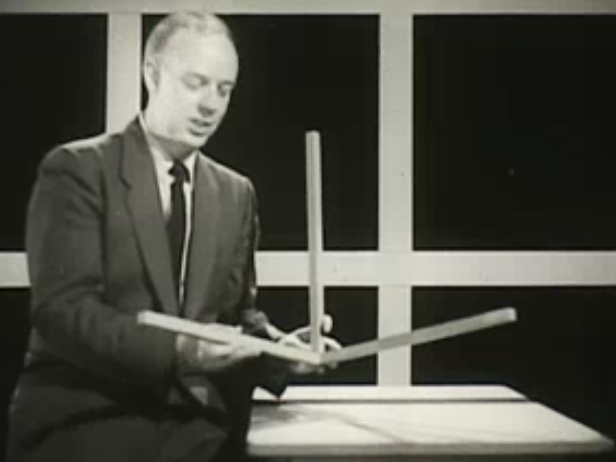
\includegraphics[width=0.5\linewidth]{prof-hume-with-an-example-frame-of-reference.png}
            \caption{Prof. Hume with a Three-dimensional Frame of Reference}
            \label{fig: a-3d-for}
        \end{figure}

Prof. Hume: This represents a ``Frame of Reference''. (Handles the model) Just three rods stuck together so that each is at right angles to the other two (places it back on the table). Now, I am going to move in this direction (points his left index finger to his right, that is, to the viewers' left; he appears moving to the left of the screen \emph{because} a grid on the wall behind him appears to move to the right of the screen.) You see the frame at the \emph{same spot} on the screen, but you know I am moving this way (points to his left with his right index finger), \emph{because} you see the wall moving this way (points to his left) \emph{behind} me. \emph{But how do you know that I am not standing still and wall moving}? (In a second, we see Prof. Ivey pushing the wall behind Prof. Hume and in fact, now Prof. Hume appears still!) It \emph{was the wall} that was moving.

(Both smile; Prof. Ivey has pushed the wall out of the view, there's a black background.) Now the wall has disappeared and you have \emph{no way} of telling whether I am moving or not! But now you know that I am moving (Prof. Ivey, leaning against the wall, appears behind Prof. Hume. Prof. Ivey, along with the wall, is moving toward the viewers' left). The point of this is ``all motion is relative.'' \textbf{In both cases, I was moving relative to the wall and the wall was moving relative to me.}

(The camera now moves to the left where Prof. Ivey is leaning against the wall.)

Prof. Ivey (has his left hand against the wall): All motion is relative, but we tend to think of one thing as being fixed and the other thing as being moving. We usually think of the Earth as fixed and walls are usually fixed to the Earth, so perhaps you were surprised the first time when it \emph{was} the wall that was moving and \emph{not} Dr. Hume. A Frame of Reference fixed to the Earth is the most common Frame of Reference in which to observe the motion of other things.

Personal commentary: When we observe things, we tend to think of us being in this most common Earth Frame of Reference. This is our usual experience. When we do our first car ride, or bus ride, or especially train ride, we clearly think of trees moving backward even though they are, by the virtue of being \emph{fixed} to the Earth, not moving. But since we are in the ``driver's position'', so to speak, we think of us being fixed (not moving) and trees moving backward.

Prof. Hume (touches the same model of 3 axes that is placed on a table): This is the Frame of Reference that you are used to. The frame is fastened to the table, the table is bolted to the floor, the floor is anchored in the building, and the building is \emph{firmly} attached to the Earth. Of course the reason for having \emph{three} rods is that the position of any object such as this ball (holds a small steel ball in front on the 3-axis model which is on his left) can be specified using these three (touches one of the rods) reference lines. (Places his right index finger on the rod straight up) This reference line points in the direction which we call ``up''. This is a different direction here than it is in the other side of the Earth.

Personal commentary: I think that by ``the other side of the Earth'' he means the southern hemisphere because I believe the ``up'' axis is pointing radially outward and, in the northern hemisphere (Canada) where I believe Prof. Hume is, that points in a direction that is different from what the ``up'' direction points to, in, say, Australia.

(Points both his hands alone the other two axes) And these two reference lines specify a plane (waves his right palm along the face of the table on which the 3-axis model is placed) which we call ``horizontal'' or ``level''. 

Prof. Hume: \textbf{In this film we are going to look at motion of objects in this ``Earth Frame of Reference'' and in other Frames of Reference moving in different ways relative to the Earth Frame} [of reference].

Well, let's look at a motion.

(Moves to another object on the same table that has a small cart to which a black vertical rod about 18 inches tall is attached that has an electromagnet at its top. He also has a steel ball.) This steel ball can be held up by the electromagnet (places the ball there). Now I am going to open a switch and you watch the motion of the ball.

(Presumably, presses a switch open which makes the electromagnet lose the magnetism and ball falls straight down. This is shown in close-up.)

Prof. Hume: The ball is accelerated straight down by gravity along a line ``parallel'' to this vertical reference line (points to the vertical rod.) 

(The cart now moves along the edge of the table to the other end where Prof. Ivey is standing. It seems that the motion of the cart is controlled electromagnetically. Prof. Ivey presses a switch and the cart comes to a halt.)

Prof. Ivey: As you can see, the electromagnet is mounted on a cart that can move (shows the direction of motion parallel to the table). Now I am going to do the exactly same experiment that Dr. Hume did, but this time, while the cart \emph{is} moving \emph{at a constant velocity}.

Personal commentary: Unlike the previous experiment wherein the cart was stationary. 

Prof Ivey: The cart is pulled along by a string which is wound around this phonograph turntable and that pulls it \emph{with constant velocity}.

(Prof. Ivey moves the cart, the electromagnet attached to it, and the steel ball to his right along the edge of the table. He reveals a short white line on the path of the cart's intended motion when it is pulled by that string.)

Prof Ivey: When the cart passes this line, the ball is released (he demonstrates that by pulling the cart to his left and the ball falls when the cart passes the line) as you can see. I am going to start the cart down at the [right] end of the table so that by the time it gets to this point (points to the white line) I can be sure it's moving with a constant velocity. And I want \emph{you to watch right here} so that you'll see the ball falling. 

(He Moves the cart to the right end of the table. He releases the cart the sound of whose rolling wheels you can hear; the cart is not in the current frame of the camera as the camera shows the white line and its surroundings in a close-up. The cart would enter the view on the viewers' left. As expected, the ball falls as the cart crosses the white line while moving with a constant velocity. The ball can be seen falling right in front of the vertical reference rod. Prof. Ivey is following along and catches the cart by his right hand. He brings it back to the white line.)

Prof Ivey: I think you can see that the ball landed in \textbf{exactly the same position that it did before} when Dr. Hume did the experiment \emph{with the cart fixed}.

\textbf{But this time, the ball could not have fallen \emph{straight down}}. Let me show you why. (He moves the cart back; the ball is in his right hand and while pulling the cart by his hand to the left as it passes the white line he catches the ball). The ball was released at that point (the ball falls and he catches it). If it had fallen straight down, because the cart moves on and [because of] the time it takes to fall, it would have landed back here somewhere (he places the ball \emph{to the left of} the vertical reference rod), but it didn't. (Moves the cart back, attaches the ball to the electromagnet) Now I am going to do the experiment again. This time, I am going to let you watch the motion through a slow-motion camera (moves a camera cart -- with an attached camera -- to the center of the table and fixes it there) which is fixed here. As the cart moves by, the ball will fall (he demonstrates how), and you can watch in the slow-motion camera (he presses a button on the fixed camera so that it starts recording).

(Now there's only camera on the screen and one can hear the cart move and see the ball fall in slow-motion as captured by the camera.)

Prof Ivey: I'll show this to you again. This time there'll be a line on the film so that you can see the path. (He does it again and one can see the path as in Figure \ref{fig: fall-of-a-constant-horizontal-velocity-ball-under-gravity}).
        \begin{figure}[h!]
            \centering
            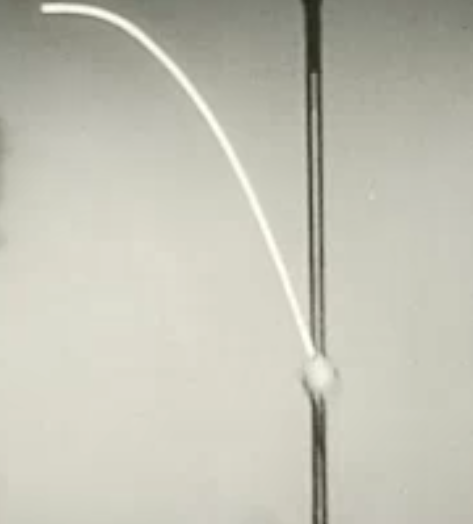
\includegraphics[width=0.7\linewidth]{fall-of-a-constant-horizontal-velocity-ball-under-gravity.png}
            \caption{Fall of a Constant Horizontal Velocity Ball Under Gravity}
            \label{fig: fall-of-a-constant-horizontal-velocity-ball-under-gravity}
        \end{figure}

I think [as you can see] that the path of the ball is a parabola. 

But all of this has been in a Frame of Reference [that is] fixed to the Earth. 

Personal commentary: Here, he should have said, "But all of this is being observed [by you] from a Frame of Reference [that is] fixed to the Earth. That is because the cart is in a Frame of Reference that is moving with a constant velocity \emph{with respect to} (or relative to) the Earth Frame of Reference where we are located and where we are observing the cart from.

Prof Ivey: How this motion \emph{looks} in a Frame of Reference which was moving along with the cart.

Personal commentary: This is normal speech, and, as such, it may have some errors. This is because the above sentence sounds ungrammatical. Maybe he meant, ``[Let's see how this motion looks \dots]''.

(Picks up a smaller model of the 3-d axes and places it on the cart) Frame of Reference like that. 

Prof Ivey: Well, so that you can see what it looks like I am going to \emph{fix} this slow-motion camera so that it moves with the cart. (While doing what he said) Like this. (The camera and the cart now move together).

I am going to do the experiment again. And incidentally I'll start it and then I am going to stand here (pointing where he currently is (in front of the video camera)) so that when the ball falls you will have something (points to himself) which is fixed, as a reference point. 

(Moves the cart-camera assembly all the way to his right, attaches the ball to the electromagnet, turns the camera switch on so that it starts recording, and stands behind the white line where we will observe the falling ball. The cart starts moving to Prof. Ivey's left and as it crosses the white line, the ball falls ``straight down''.)

Prof Ivey: In the ``moving Frame of Reference'' I think you can see that the path of the ball is a vertical straight line (he points to a fictitious line in front of the reference rod that connects the electromagnet to the cart). It looks exactly the same as it did before when Dr. Hume did the experiment \emph{with the cart fixed}.

\textbf{If we were moving along in this Frame of Reference and we couldn't see the surroundings then we wouldn't be able to tell \emph{by this experiment} that we were [cart was] moving at a constant velocity. As a matter of fact, we wouldn't be able to tell by \emph{any experiment} that we were [cart was] moving at a constant velocity.}

Personal commentary: This trick of seeing things through a slow-motion camera that is placed in a Frame of Reference of interest is very effective! I have wondered several times how one can actually comment on certain motions that are occurring in Frames of Reference that are moving with respect to our Earth Frame of Reference. This idea of making a camera which records the motion \emph{stick to the Frame of Reference of interest} is exactly what I was missing back in my school/college days!

Prof Ivey: I am going to do the experiment once more, and this time, I am \emph{not} going to stand here behind the ball as it falls, so that you \emph{won't} have any fixed reference frame.

(Takes the cart-camera assembly to starting position and releases it. The cart moves, the ball falls straight down (we are viewing this through the attached slow-motion camera), but this time there is nothing fixed to compare it against.)

Personal commentary: Since \emph{everything} we saw in that last experiment was in a Frame of Reference that was moving at a constant velocity relative to the Earth Frame of Reference, there was no way for us to tell whether or not everything was at rest or moving!

(Now Prof. Ivey is standing behind the cart)

Prof. Ivey: As far as you are concerned, that time, the cart wasn't necessarily moving at all. That time, when you couldn't see the background, then it was perhaps harder for you to realize that you were in a moving Frame of Reference. 

Personal commentary: Here ``you'' means the camera because the camera is observing (and recording) the moving cart's motion and since it is fixed to the cart, the camera \emph{is} in a moving Frame of Reference.

Prof. Ivey: The important thing to realize here is that all Frames of Reference moving at\footnote{The time-stamp here is 08.48.} constant velocity with respect to one another are equivalent.

Personal commentary: He should have said, ``\dots moving at \emph{the same} constant velocity \emph{with respect to another Frame of Reference} are equivalent.'' The statement ``\dots all Frames of Reference moving at constant velocity with respect to one another are equivalent'' is ambiguous. First of all, if they are moving at some constant velocities that are not the same (same direction and same magnitude), then they are not equivalent. Secondly, it does not make sense to say that equivalent Frames of Reference are moving at a constant velocity do so with respect to each other. For example, if a train A moves at a constant speed of $5\si{\m\per\s}$ in some direction and another train B moves in the same direction at a constant speed of $10\si{\m\per\s}$, then their respective Frames of Reference are clearly not equivalent. But if they are moving at the same constant velocity with respect to another Frame of Reference, say, the Earth Frame of Reference, then they are equivalent; it does not matter if you are on train A or train B when you observe motions of objects -- those motions will all look the same, making the train A Frame of Reference and train B Frame of Reference equivalent.

Prof. Hume: Dr. Ivey showed you what the motion of the ball that was released from the moving cart looks like in the Earth Frame of Reference and in the cart Frame [of Reference].

Personal commentary: Till now, we have done three experiments:
\begin{enumerate}
    \item \label{item: exp1} Ball is released from a cart that is fixed in the Earth Frame of Reference. The motion is also observed from the same Earth Frame of Reference.
    \item \label{item: exp2} Ball is released from a cart that is moving at a constant velocity with respect to the Earth Frame of Reference. The motion is observed from the Earth Frame of Reference.
    \item \label{item: exp3} Ball is released from a cart that is moving at a constant velocity with respect to the Earth Frame of Reference. The motion is observed from the cart Frame of Reference (by a camera).
\end{enumerate}

Prof. Hume: The motion looks simpler from the cart. 

Personal commentary: Here ``simpler'' is subjective. What he means is that the motion in 2) above (a parabola) is slightly more difficult to observe clearly than the motion in 3) above (a straight line) when the observer (the camera) is attached to the cart.

Prof. Hume: (He stands by a black box with a circular disk that has a small white circular spot on it) Now I want you to watch the motion of this white spot (points to it) (See Figure \ref{fig: prof-hume-cycloid-1}).
        \begin{figure}[h!]
            \centering
            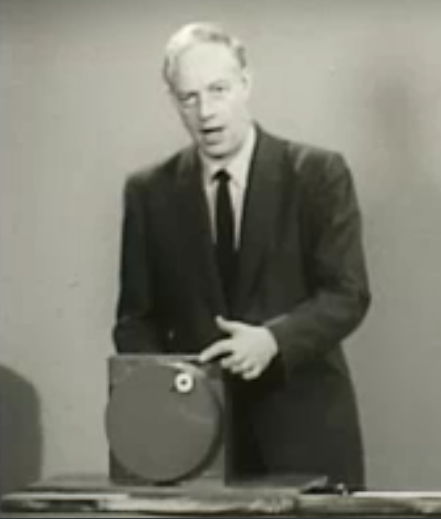
\includegraphics[width=0.7\linewidth]{prof-hume-cycloid-1.png}
            \caption{Motion of a Point on a Rolling Wheel}
            \label{fig: prof-hume-cycloid-1}
        \end{figure}

(He presses a switch and the black box starts sliding (apparently with constant velocity) along the table. The circular disk starts rotating. Since the disk is fitted to the box that slides, the disk is both rotating and sliding. So does the white spot whose motion we are observing.)

Prof. Hume: You probably see the spot moving in a circle. 

(He lets the disk roll for a few seconds and the motion of the white spot is traced behind as shown in Figure \ref{fig: prof-hume-cycloid-2}.)
        \begin{figure}[h!]
            \centering
            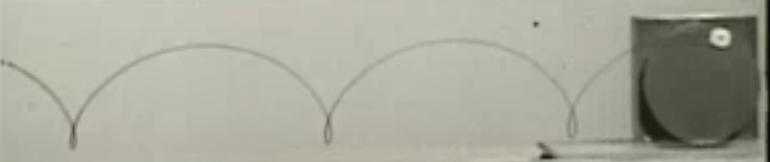
\includegraphics[width=0.7\linewidth]{prof-hume-cycloid-2.png}
            \caption{The Path Traced by a Point on a Rolling Wheel}
            \label{fig: prof-hume-cycloid-2}
        \end{figure}

Prof. Hume (Shows the cycloid traced on the screen): But this is what its path is actually like, in [the] Earth Frame of Reference. This [the Earth Frame of Reference] is your ``normal'' Frame of Reference. You saw the spot moving in a circle, \emph{because your eye moved along with the cart}. \textbf{You put yourself in the Frame of Reference of the moving cart}. 

\emph{So you see, it isn't always true that we view motion from the Earth Frame of Reference}. When the motion is \emph{simpler} from the moving frame, you automatically put yourself in that moving frame! 

Personal commentary: They should have shown it the same way as in experiment 3) above by attaching a slow-motion camera to the moving block. The camera would then see the spot only move in a circle. The motion of the spot in the Earth Frame of Reference is a cycloid. 

(Now we see Prof. Ivey and Prof. Hume sitting across a table with a smooth glass surface. Prof. Ivey holds an object mounted on something that looks like a metal puck.)

Prof. Ivey: Now we are going to do another experiment on relative motion to show \emph{how to compare the velocity of an object in one Frame of Reference to its velocity in another Frame of Reference}.

If I give this dry ice puck\footnote{It has dry ice (solid \ce{CO2}) which evaporates readily reducing the friction between the surfaces.} a certain start (gently pushes the puck toward Prof. Hume sitting right across), it moves straight across the table with a speed which is essentially constant because the forces of friction have been made very small. This is just the ``Law of Inertia'': An object [that is not at rest] moves with a constant velocity unless an unbalanced force acts on it. 

Prof. Ivey (to Prof. Hume): Now if you could give it the same start backwards \dots

Prof. Hume (Complies): Okay.

Prof. Ivey (Catches the puck): If Dr. Hume gives it the same start it moves back in this (pointing toward himself) direction with the same velocity.

Now we are on a car here, a car which can move and which really is going to move in this (points toward Dr. Hume) direction and we are going to repeat the experiment. Alright, let's go.  

(Prof. Ivey gives a start to the puck toward Prof. Hume. The wall behind them appears to move backward at the same time -- this is quite evident if we focus on a grid intersection point which is seen moving to \emph{our} left. Prof. Hume sends the puck back to Prof. Ivey.)

Personal commentary: The video camera (that is, the viewer) is on the same car as the professors and the table; the wall isn't. This is why we are able to see the professors fixed (they are stationary relative to the camera), the puck move (it is actually moving in the same Frame of Reference as the camera) to Prof. Hume, and the wall move backward (it is in the Earth Frame of Reference relative to which the camera is moving forward and which is moving backward relative to the camera). 

Prof. Ivey (Catches the puck): If we were making measurements here, then we'd observe the same velocity, that is the same experimental result that we did before, and so would you, because you are observing this experiment through a camera which is fixed to this car. That is, you are in a ``moving Frame of Reference'' [along] with us. But now we are going to do the experiment again and this time you watch through a camera which is fixed in the Earth Frame of Reference.

(Now the same car appears. The professors, the table, and the puck start moving to the right, the wall starts moving to the left.)

Prof. Ivey (Gives the puck a start): Now concentrate on watching the puck, don't let your eye follow us. And I think you'll see that \textbf{it'll move faster that way} (points to Prof. Hume) \textbf{and not so fast this way} (points toward himself; at the same time, Prof. Hume gives the puck a start back) \textbf{relative to you and relative to the wall behind}.

(Prof. Ivey pushes the cart to Prof. Hume and darts off to a blackboard and begins writing on it).

Prof. Ivey: Here is the cart (starts drawing a schematic diagram of the arrangement that they were experimenting with) which was moving along this direction (points to the viewers' right) with a velocity $u$. We were sitting on the car at a table; here I am over on this side and Dr. Hume was on this side. And we were pushing this puck back and forth on the table. When I pushed it went in this direction (points to the right) with a velocity $v$. When Dr. Hume pushed, it went in this direction (points to the left) with \emph{the same} velocity $v$. But this is the velocity \emph{relative to the car}. What about the velocity relative to an observer on the ground in the fixed frame? Well, if it is pushed in this direction (points to the right) its velocity is $u+v$. If it's in this direction (points to the left), its velocity is $u-v$. (He gradually completes the Figure \ref{fig: prof-ivey-explains-relative-motions}).
        \begin{figure}[h!]
            \centering
            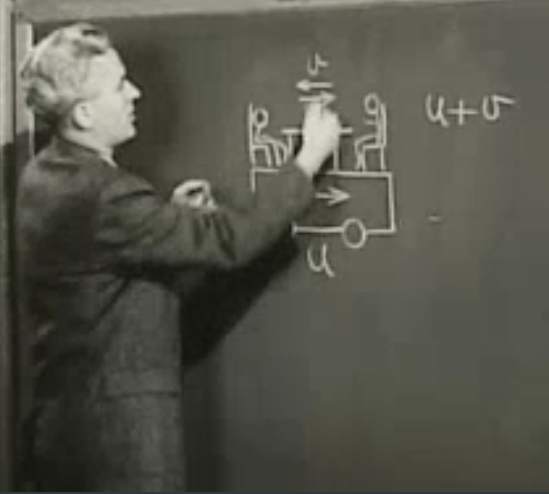
\includegraphics[width=0.5\linewidth]{prof-ivey-explains-relative-motions.png}
            \caption{Prof. Ivey Explains Relative Motions Across Frames of Reference}
            \label{fig: prof-ivey-explains-relative-motions}
        \end{figure}

Prof. Ivey: This is all very reasonable; there's nothing very hard to understand here. The surprising thing about this expression (points to $u\pm v$) is that it is \emph{not} accurate in \emph{all circumstances}. At very high speeds -- and by high speeds I mean speeds close to the speed of light -- this expression breaks down. At these very high speeds we have to use the ideas about relative motion developed by Albert Einstein in his special theory of relativity. However, for all the speeds that we are ever likely to run into, this expression -- $u\pm v$ -- is completely adequate. 

Prof. Hume: So far, we've been talking about Frames of Reference moving at a constant velocity relative to one another. Now I am going to do the experiment with the dropping ball again; only this time, the cart \emph{will be accelerated} relative to the Earth Frame [of Reference].

Personal commentary: The point is subtle: the cart is now going to be \emph{accelerated} which means its velocity will be changing, rather than being constant.

(This time the cart is attached to falling weights that Prof. Hume points to.)

Prof. Hume (Points to weights): These weights will fall and give the cart a constant acceleration. (Walks back to the cart and the electromagnet and places the ball up there). I put the ball up and then I'll release that the motion is very fast and I want you to watch at the point where the ball is released from the fixed camera. 

Personal commentary: I can't believe he said ``from the fixed camera''. The ball is released from the fixed electromagnet, so that sounds like a slip of tongue that should've been caught during the editing of the film! 

Prof. Hume (Moves rightwards to the cart attached to the weights) : Ready? 

(Lets the cart go. The cart moves to our right very fast and it's hard to spot the falling ball.)

Prof. Hume (Comes running where the cart has been stopped by a stopper; we see a ball fall in [what looks like] a parabola just like before): I don't know if you saw that or not, but the path of the ball was the same as it was before (experiment \ref{item: exp2}, Figure \ref{fig: fall-of-a-constant-horizontal-velocity-ball-under-gravity}). Only this time it landed in a \emph{different spot} (See Figure \ref{fig: ball-falls-off-an-accelerating-cart}). 

\begin{figure}
    \centering
    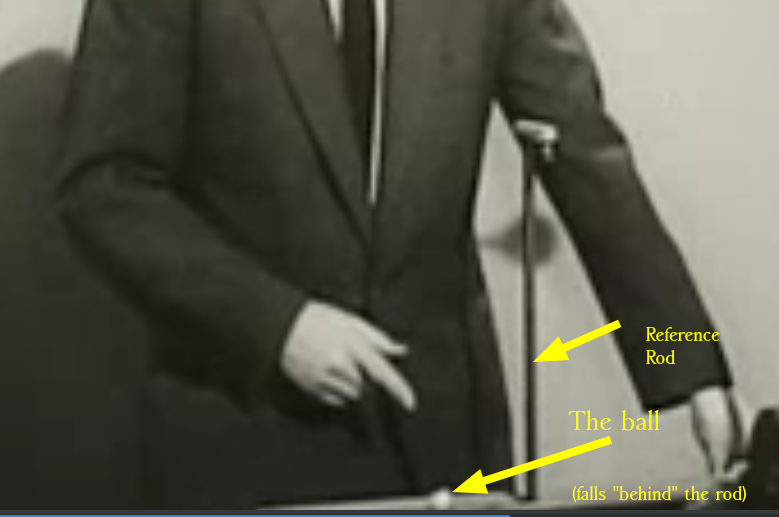
\includegraphics[width=0.7\linewidth]{ball-falls-off-an-accelerating-cart.png}
    \caption{Ball Falls off an Accelerating Cart and Lands Behind the Rod}
    \label{fig: ball-falls-off-an-accelerating-cart}
\end{figure}


This is because the cart kept on accelerating in this direction (points to his left) as the ball was falling (points vertically downward).

Now I am going to let you see it again with the slow-motion camera fixed onto the cart.

Personal commentary: Just now we saw the cart -- from the Earth Frame of Reference -- race to our right. 

(Prof. Hume slides the cart back to its starting position, attaches the ball back up, fixes the slow-motion camera to the cart, and lets the cart-camera assembly go. Through the slow-motion camera, we see the ball landing behind the rod. See Figure \ref{fig: detached-ball-lands-behind-an-accelerating-cart}).

\begin{figure}
    \centering
    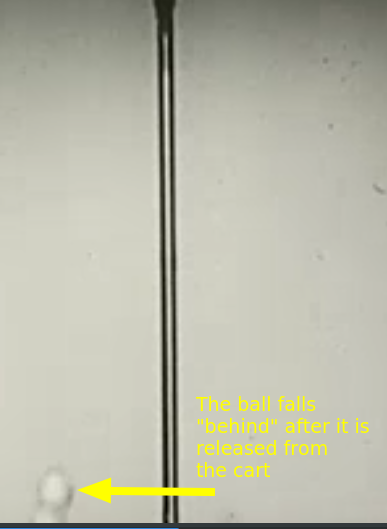
\includegraphics[width=0.7\linewidth]{detached-ball-lands-behind-an-accelerating-cart.png}
    \caption{The Lagging Ball's Motion as Seen Through a Slow-motion Camera}
    \label{fig: detached-ball-lands-behind-an-accelerating-cart}
\end{figure}

Prof. Hume: This time you saw the ball moving off to one side (traces the balls ``backward'' motion with his hand). And not following down the vertical reference line as it did in the constant velocity case (\ref{item: exp3}).

Now suppose you were in this accelerated Frame of Reference, how could you explain this (points to the fictitious line in which the ball falls and lands behind the rod) motion?

Personal commentary: Technically, when we saw, through the camera, the ball fall, we \emph{were} in that accelerated Frame of Reference because the camera is attached to the cart that accelerates. To say that the ``cart accelerates'' is equivalent to say that the ``cart is \emph{in} an accelerated Frame of Reference'' (relative to ``our'' Frame of Reference which is ``fixed'').

(Prof. Hume walks toward a blackboard where a schematic diagram of the cart's motion is already drawn (See Figure \ref{fig: prof-hume-interprets-non-inertial-frame}).)

        \begin{figure}[h!]
            \centering
            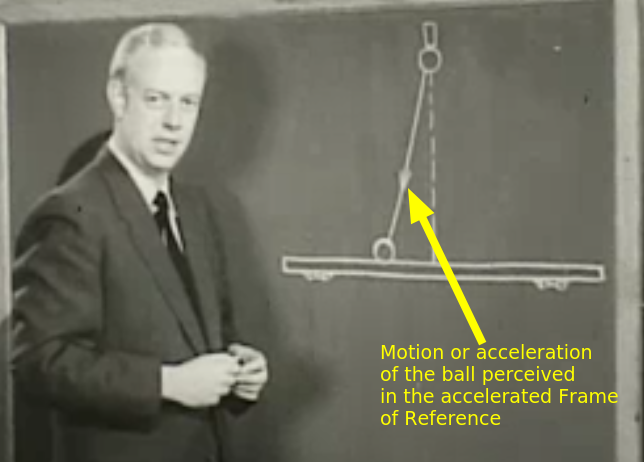
\includegraphics[width=0.5\linewidth]{prof-hume-interprets-non-inertial-frame.png}
            \caption{Prof. Hume Interprets a Non-inertial Frame of Reference}
            \label{fig: prof-hume-interprets-non-inertial-frame}
        \end{figure}

Prof. Hume (Stands by the blackboard): Gravity is the only force acting on this ball (points to the ball in the diagram of Figure \ref{fig: prof-hume-interprets-non-inertial-frame}). So it should fall straight down. But if the ``Law of Inertia'' is to hold, there must be a force pushing sideways on the ball in this direction (points to the ball's apparent motion through the camera in which the ball \emph{lands behind the rod}) to cause it to deviate from the vertical path. \textbf{But what kind of force is it?} It isn't a gravitational, or an electric, or a nuclear force. In fact, it isn't a force at all as we know one! So we are left to conclude that it, since there \emph{is no force} that could be pushing in this direction on the ball, the ``Law of Inertia'', \emph{just does not hold}! \textbf {This is a strange Frame of Reference}. 

\textbf{We call a Frame of Reference in which the ``Law of Inertia'' holds an ``Inertial Frame [of Reference]''. The Law of Inertia holds in the Earth Frame of Reference. So it is an inertial frame. The cart, moving at a constant velocity relative to the Earth is [also] an inertial frame. But the cart which is accelerated [relative to the Earth] is not an inertial frame.}

Because the Frame of Reference that we're used to living in, is one in which the ``Law of Inertia'' holds, when we go into a ``Non-inertial Frame'', like the frame of the accelerated cart, \textbf{our belief in the ``Law of Inertia'' is so strong that when we see the acceleration} [I think he should've said ``motion''] \textbf{sideways,} (a picture of the ball falling backward appears) \textbf{we think there is a force causing it. So we make up a fiction that there \emph{is} a force. And sometimes we call it a ``fictitious force''.}

Fictitious forces arise in accelerated Frames of Reference. The frame is accelerated in this direction (points forward) so, you, in the frame, see the acceleration [motion] in this direction (points backward) and you say that there is a force causing it. 
\end{document}
